\pdfoutput=1
\documentclass[11pt,a4paper]{article}

% ---- Packages ----
\usepackage[utf8]{inputenc}
\usepackage[T1]{fontenc}
\usepackage{lmodern}
\usepackage{microtype}
\usepackage{amsmath,amssymb,amsthm,mathtools}
\usepackage[a4paper,margin=1in]{geometry}
\usepackage{xcolor}
\usepackage[unicode,colorlinks=true,linkcolor=blue,citecolor=blue,urlcolor=magenta]{hyperref}
\usepackage[nameinlink,capitalize]{cleveref}
\usepackage{booktabs}
\usepackage{siunitx}
\usepackage[section]{placeins}
\sisetup{group-separator={\,},detect-all}
\usepackage{pgfplots}
\pgfplotsset{compat=1.17} % arXiv-safe (slightly older than 1.18)
\usetikzlibrary{positioning,arrows.meta,shapes,calc}
\usepackage{graphicx}

% avoid overfull boxes
\setlength{\emergencystretch}{3em}

% Disable math macros inside PDF bookmarks
\pdfstringdefDisableCommands{%
  \def\gap{lambda2}%
  \def\hdeg{hdeg}%
  \def\nL{L}%
}

% ---- Theorem environments ----
\newtheorem{theorem}{Theorem}
\newtheorem{lemma}{Lemma}
\newtheorem{proposition}{Proposition}
\newtheorem{conjecture}{Conjecture}
\theoremstyle{remark}
\newtheorem*{remark}{Remark}

% ---- Macros ----
\newcommand{\nL}{\mathcal{L}}
\newcommand{\gap}{\lambda_2}
\newcommand{\hdeg}{\widehat{\deg}}

% ===== TITLE =====
\title{\textbf{Spectral Predictors for Tseitin Hardness:\\
A Physics-Motivated Exploration}\\
\large Preliminary Conjectures and Empirical Observations}

\author{\textbf{Amandine Morin}%
\footnote{Research conducted independently.}%
\footnote{No institutional affiliation.}}

\date{Revised February 2026}

\begin{document}
\maketitle

\begin{center}
\small
\textcolor{red}{\textbf{EXPLORATORY PREPRINT — NOT PEER-REVIEWED}}\\[0.5em]
\textcolor{blue}{This work presents \textbf{conjectures and preliminary observations}
on spectral predictors for proof complexity. No new theorems are proved.
Empirical validation is limited to small illustrative instances ($n \leq 80$).
This document invites discussion, testing, and critique.}
\end{center}

\begin{abstract}
We explore a physics-first viewpoint on propositional proof complexity, motivated by
Landauer's principle~\cite{Landauer1961}: information processing has an inherent physical cost.
For Tseitin contradictions over quasi-regular graphs~\cite{Tseitin1968,KrajicekBook}, we argue
that any solver must process a minimal amount of \emph{structural information} depending jointly
on local density and global connectivity.

We introduce the predictor
\[
\hdeg(G) := \frac{n}{\sqrt{1/d + 1/\gap}},
\]
where $n$ is the number of vertices, $d$ the average degree, and $\gap$ the second-smallest
eigenvalue of the normalized Laplacian~\cite{Chung1997}.
We formulate corresponding Kolmogorov-type information conjectures~\cite{LiVitanyi},
conjectural decision-tree lower bounds reflecting expansion~\cite{HooryLinialWigderson},
and a link to Polynomial Calculus degree~\cite{Razborov1998}.
Empirical data (embedded PGFPlots) suggests a qualitative correlation between $\hdeg(G)$ and
practical SAT-solving time on Tseitin formulas.
% ---- UPDATED (minimal) ----
In addition, we report updated controlled experiments obtained using a reproducible C++ pipeline
and the Kissat CDCL solver, highlighting a sharp structure-dependent transition in solver behavior at fixed $(n,d)$
under Watts--Strogatz rewiring.

\medskip
\noindent\textbf{Note.} This is an exploratory preprint presenting conjectures and
preliminary empirical validation. No new theorems are proved. We explicitly invite
the community to test, refine, or refute these hypotheses.
\end{abstract}

\paragraph{Contributions.}
This exploratory work offers:
\begin{itemize}
  \item A physics-motivated \emph{conjectural} framework (MPCC) linking spectral structure
        to proof complexity for Tseitin formulas;
  \item A simple predictor $\hdeg(G)$ calibrated on canonical graph families
        (cycles, grids, expanders, completes);
  \item Preliminary empirical evidence that $\hdeg(G)$ correlates with CDCL solving time
        on small Tseitin instances;
  \item A roadmap of conjectures connecting decision-tree complexity, Polynomial Calculus,
        and time-bounded Kolmogorov complexity.
\end{itemize}
\textbf{No new theorems are proved.} All formal lower-bound statements are explicitly
presented as conjectures.

% ============================
\section{Introduction}

The cost of distinguishing SAT from UNSAT is fundamentally informational.
A solver must extract, manipulate, and retain a minimal volume of structural information
about the instance. Following Landauer's principle~\cite{Landauer1961}, we take seriously
the idea that this informational cost has a structural footprint in the input.

Tseitin contradictions~\cite{Tseitin1968,KrajicekBook} are among the canonical hard families
in propositional proof complexity. They encode parity constraints on a graph $G$ and are
unsatisfiable exactly when the total charge is odd. On expander graphs, Tseitin formulas
yield strong lower bounds in Resolution~\cite{BenSassonWigderson2001} and algebraic systems
such as Polynomial Calculus (PC)~\cite{Razborov1998}.

Meanwhile, spectral graph theory~\cite{Chung1997,HooryLinialWigderson} provides a robust way
to quantify connectivity via the spectrum of the normalized Laplacian, with the spectral gap
$\gap$ tightly related to edge expansion and mixing.

In this preprint we propose a structural predictor,
\[
\hdeg(G) = \frac{n}{\sqrt{1/d + 1/\gap}},
\]
combining local density ($d$) and global connectivity ($\gap$) in a harmonic fashion.
We conjecture that $\hdeg(G)$ approximates the minimal information budget that any
reasoning process must handle to refute $\mathrm{Tseitin}(G,\chi)$.
We phrase this in time-bounded Kolmogorov terms~\cite{LiVitanyi} and
as conjectured lower bounds in decision-tree and algebraic proof models.

Our goal here is not to present a complete lower-bound proof, but to propose a coherent
structural scale that can be probed both analytically and empirically, and which appears
to interpolate naturally between known behaviors on cycles, grids, expanders and dense graphs.

Even when the degree is fixed, the global geometry of the constraint graph can vary
significantly depending on the generation model, as illustrated in
Figure~\ref{fig:graph_models_contrast}.

\begin{figure}[ht]
  \centering
  \includegraphics[width=0.48\linewidth]{figures/circulant_n80_d4_s0.png}\hfill
  \includegraphics[width=0.48\linewidth]{figures/config_n80_d4_s3.png}
  \caption{
  Degree-regular graphs with identical parameters ($n=80$, $d=4$) generated using two
  different models.
  \textbf{Left:} circulant graph (highly symmetric, homogeneous geometry).
  \textbf{Right:} configuration-model graph (irregular geometry with local bottlenecks).
  Despite identical degree sequences, the resulting structures differ substantially at the geometric level.
  }
  \label{fig:graph_models_contrast}
\end{figure}
\FloatBarrier

% ============================
\section{Graphs, spectrum, and conventions}

Let $G=(V,E)$ be a simple graph with $|V|=n$ and average degree $d$.
The normalized Laplacian is
\[
\nL = I - D^{-1/2} A D^{-1/2},
\]
with eigenvalues
\[
0 = \lambda_1 \le \gap \le \cdots \le \lambda_n \le 2,
\]
where $\gap$ is the second-smallest eigenvalue (the spectral gap)~\cite{Chung1997}.

\begin{remark}[Cheeger inequality]
Let $\phi(G)$ denote edge conductance.
Cheeger-type inequalities for the normalized Laplacian~\cite{Chung1997} give
\[
\frac{\phi(G)^2}{2} \le \gap \le 2\phi(G),
\]
supporting the use of $\gap$ as a proxy for expansion.
\end{remark}

We focus on quasi-regular families (bounded ratio between maximum and minimum degrees),
and we view $G$ as the constraint graph of a Tseitin formula~\cite{Tseitin1968,KrajicekBook}.

% ============================
\section{MPCC and Kolmogorov formulation}

We now phrase the Minimal Proof Compression Conjecture (MPCC) and a
Kolmogorov-based variant.

\begin{conjecture}[MPCC]\label{conj:mpcc}
For any quasi-regular family of graphs, any solver deciding $\mathrm{Tseitin}(G,\chi)$
must process at least
\[
c\cdot \frac{n}{\sqrt{1/d + 1/\gap}}
\]
bits of structural information about $G$, for some constant $c>0$, robust under
preprocessing and natural re-encodings.
\end{conjecture}

\paragraph{Kolmogorov formulation.}
Following Li--Vitányi~\cite{LiVitanyi}, let $K^t$ denote time-bounded Kolmogorov
complexity with side information. For a canonical encoding $\mathrm{enc}(G)$, set
\[
K^t(G \mid (n,d,\gap))
=\min\{|p| : U(p,(n,d,\gap)) = \mathrm{enc}(G) \text{ in time } \le t(|G|)\}.
\]

\begin{conjecture}[Kolmogorov--MPCC]\label{conj:kmpcc}
There exist $c>0$ and a polynomial $t(\cdot)$ such that for all quasi-regular graphs~$G$,
\[
K^t(G \mid (n,d,\gap))
\;\ge\;
c \cdot \frac{n}{\sqrt{1/d + 1/\gap}} - o(n).
\]
\end{conjecture}

% ============================
\section{Decision-tree lower bounds}

We informally sketch a decision-tree model for refuting Tseitin contradictions and
formulate our lower-bound claims as conjectures, since a fully detailed proof is not
included in this preprint.

Let $\mathrm{R}_0^{\mathrm{DT}}(G)$ denote the zero-error randomized decision-tree
complexity of refuting $\mathrm{Tseitin}(G,\chi)$, where each query requests local
information about edges and incident constraints.

\begin{conjecture}[DT lower bound for $d=O(1)$]\label{conj:dt}
For any bounded-degree quasi-regular graph $G$, there exists $c>0$ such that
\[
\mathrm{R}_0^{\mathrm{DT}}(G) \;\ge\; c\, n\sqrt{\gap}.
\]
\end{conjecture}

\begin{conjecture}[Harmonic-bound template]\label{conj:harm}
For any quasi-regular graph $G$, there exists $c>0$ such that
\[
\mathrm{R}_0^{\mathrm{DT}}(G)
\;\ge\;
c \cdot \frac{n}{\sqrt{1/d + 1/\gap}}.
\]
\end{conjecture}

These conjectures are motivated by Yao-style arguments and the behavior of
expander graphs~\cite{HooryLinialWigderson}.

% ============================
\section{Polynomial Calculus connections}

Polynomial Calculus (PC) is an algebraic proof system where propositional formulas
are translated into polynomial equations over a field and refutations proceed by
algebraic derivations~\cite{Razborov1998,KrajicekBook}. For Tseitin contradictions
over expanders and fields of characteristic not equal to $2$, Razborov~\cite{Razborov1998}
proved linear lower bounds on PC degree.

These results fit the qualitative picture suggested by $\hdeg(G)$: stronger expansion
implies higher degree, and thus higher algebraic complexity.

\begin{conjecture}[PC-degree $\Rightarrow$ touch complexity]\label{conj:pc-touch}
If $\deg_{\mathsf{PC}}(\mathrm{Tseitin}(G)) \ge r$ then
\[
\mathrm{Touch}_{\mathsf{PC}}(G) \;\ge\; c r
\]
for some absolute constant $c>0$, where $\mathrm{Touch}_{\mathsf{PC}}(G)$ is a
suitable measure of how many constraint occurrences any PC derivation must ``touch''.
\end{conjecture}

We expect $\mathrm{Touch}_{\mathsf{PC}}(G)$ to scale with $\hdeg(G)$, linking
PC-degree lower bounds to the MPCC perspective.

% ============================
\section{Calibrating the predictor $\hdeg(G)$}

We define
\[
\hdeg(G) := \frac{n}{\sqrt{1/d + 1/\gap}}.
\]

This form matches natural scales on standard graph families~\cite{Chung1997,HooryLinialWigderson}:

\begin{center}
\renewcommand{\arraystretch}{1.05}\small
\begin{tabular}{lcccc}
\toprule
Family          & $d$   & $\gap$           & $\hdeg(G)$        & Comment        \\
\midrule
Cycle $C_n$     & 2     & $\Theta(1/n^2)$ & $\Theta(1)$       & 1-D weak       \\
Grid $m\times m$& $O(1)$& $\Theta(1/n)$   & $\Theta(\sqrt{n})$& 2-D medium     \\
Expander        & $O(1)$& $\Theta(1)$     & $\Theta(n)$       & strong         \\
Complete $K_n$  & $n$   & 1               & $\Theta(n)$       & dense          \\
\bottomrule
\end{tabular}
\end{center}

% ============================
\section{Empirical sanity checks}

We test the alignment between $\hdeg(G)$ and practical SAT difficulty for Tseitin CNFs.
Families include cycles $C_n$, grids, complete bipartite graphs, and random regular graphs.
CNFs are generated by constructing $G$ and encoding XOR constraints at each vertex into
3-CNF using auxiliary variables.

% ---- UPDATED (new minimal subsection) ----
\subsection*{Updated experimental pipeline and sharp structure dependence (2026)}

We use a reproducible C++ pipeline (CNF byte-level hashing via \texttt{cnf\_hash}) 
and run Kissat under fixed resource limits, recording SAT/UNSAT/timeout outcomes.

At fixed size $n=80$ and degree $d=4$, we observe strong structure dependence even at constant $(n,d)$.
In addition to contrasts between circulant and configuration-model generators, the Watts--Strogatz experiment
below exhibits an especially sharp transition as a function of the rewiring probability $p$.

\begin{table}[h]
\centering\small
\caption{Controlled Tseitin instances at fixed size ($n=80$, $d=4$) using Kissat 
with a \SI{60}{\second} timeout (same solver and limits across generators).}
\begin{tabular}{lcccc}
\toprule
Graph family & Seeds & Result & Runtime & Comment \\
\midrule
Circulant & multiple & UNSAT & \SI{\sim12}{\milli\second} & consistently easy \\
Configuration model & multiple & timeout & \SI{60}{\second} & consistently hard \\
\bottomrule
\end{tabular}
\end{table}

\subsection*{Reproducible pipeline and a Watts--Strogatz transition (2026)}

We now detail a Watts--Strogatz experiment implemented in this pipeline.
It generates the constraint graph, builds the corresponding Tseitin CNF, 
computes a byte-level hash of the DIMACS file (\texttt{cnf\_hash}), and invokes Kissat under fixed resource limits.
Instance generation is deterministic given $(n,d,\texttt{seed},\texttt{graph\_mode},p)$,
and we record solver outcomes (SAT / UNSAT / timeout) with wall-clock runtimes.
Timeouts are defined as runs reaching the \SI{60}{\second} wall-clock limit (exit code 124 in our wrapper).

\paragraph{Watts--Strogatz experiment.}
At fixed size $n=80$ and degree $d=4$, we generate $d$-regular graphs using the
Watts--Strogatz rewiring model with parameter $p \in [0,1]$, and run Kissat with a
\SI{60}{\second} timeout. For each $p$, we run 20 distinct seeds (\texttt{seed}=0,\dots,19).
All generated instances correspond to Tseitin contradictions with odd total charge and are UNSAT by construction.

\paragraph{Observation: sharp hardness transition.}
We observe a striking structure-dependent transition with three regimes: for $p=0$ (circulant baseline),
instances are refuted quickly; for $p=0.01$ the runtime distribution becomes heavy-tailed;
and from $p\ge 0.05$ onward, \emph{all} runs hit the \SI{60}{\second} timeout under the same solver
and limits. This suggests a sharp transition from an easily exploitable geometry to a regime
where CDCL heuristics stall.

\begin{table}[h]
\centering\small
\caption{Sharp solver-behavior transition for Watts--Strogatz Tseitin instances at $n=80$, $d=4$ 
under Kissat with a \SI{60}{\second} timeout (20 seeds per $p$).}
\label{tab:ws_transition_n80_d4}
\begin{tabular}{lrrrrr}
\toprule
$p$ & runs & timeouts & timeout rate & median (\si{\milli\second}) 
& q90 (\si{\milli\second}) \\
\midrule
0    & 20 & 0  & 0.000 & 11   & 17 \\
0.01 & 20 & 1  & 0.050 & 2606 & 17870 \\
0.05 & 20 & 20 & 1.000 & 60000 & 60000 \\
0.10 & 20 & 20 & 1.000 & 60000 & 60000 \\
0.20 & 20 & 20 & 1.000 & 60000 & 60000 \\
0.50 & 20 & 20 & 1.000 & 60000 & 60000 \\
1.00 & 20 & 20 & 1.000 & 60000 & 60000 \\
\bottomrule
\end{tabular}
\end{table}
\FloatBarrier

\begin{figure}[h]
\centering
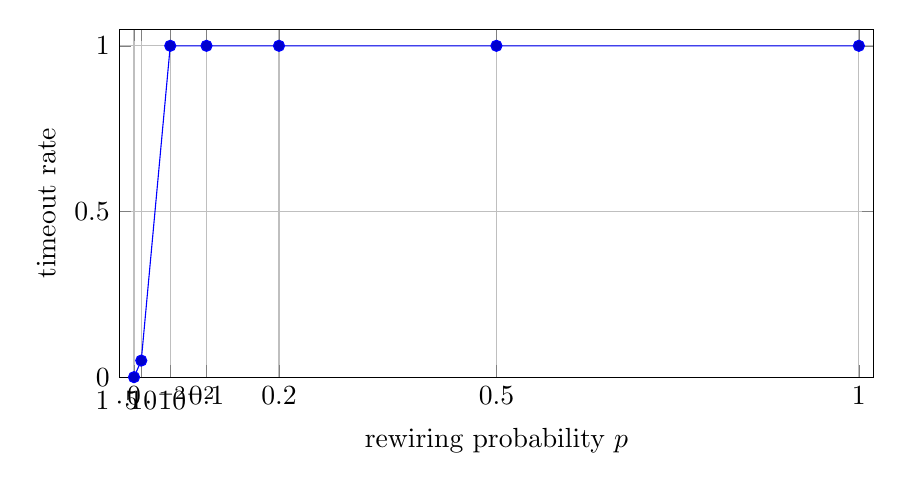
\begin{tikzpicture}
\begin{axis}[
    width=0.92\linewidth,
    height=6cm,
    xlabel={rewiring probability $p$},
    ylabel={timeout rate},
    ymin=0, ymax=1.05,
    grid=major,
    xtick={0,0.01,0.05,0.1,0.2,0.5,1.0},
    xmin=-0.02, xmax=1.02,
]
\addplot+[mark=*] coordinates {
 (0,0.0)
 (0.01,0.05)
 (0.05,1.0)
 (0.1,1.0)
 (0.2,1.0)
 (0.5,1.0)
 (1.0,1.0)
};
\end{axis}
\end{tikzpicture}
\caption{Observed timeout rate for Watts--Strogatz Tseitin instances at $n=80$, $d=4$ under Kissat with a \SI{60}{\second} limit (20 seeds per $p$).}
\label{fig:ws_timeout_rate}
\end{figure}
\FloatBarrier


\subsection*{Experimental setup and reproducibility}

We distinguish between legacy MiniSat-based illustrative experiments
and the updated Kissat-based controlled pipeline introduced above.
The experiments are illustrative rather than benchmark-oriented.
A Python script generates the graph, encodes Tseitin constraints, and invokes a
MiniSat binary with default settings. Wall-clock times are measured with a
high-resolution timer and reported in seconds; very small instances naturally round
to \texttt{0.0000} at the displayed precision.

A fully reproducible setup would fix and document:
\begin{itemize}
  \item the exact MiniSat version and compilation flags;
  \item the seeds used to generate random regular graphs;
  \item the hardware and OS environment.
\end{itemize}
% ---- UPDATED (minimal: no longer "future version intended") ----
The repository now includes an updated C++ pipeline and raw experimental outputs for reproduction,
while the legacy Python/MiniSat results below are retained as small illustrative data.

\subsection*{Dataset table}

\begin{table}[h]
\centering\small
\caption{Tseitin CNFs: measures and predictor $\hdeg(G)$.}
\begin{tabular}{lrrrrr}
\toprule
Family         & $n$ & clauses & width & $\hdeg(G)$ & time\_s \\

\midrule
cycle          &  8  &   40    & 3     & 4.044      & 0.0000 \\
cycle          & 16  &   80    & 3     & 4.333      & 0.0000 \\
cycle          & 32  &  160    & 3     & 4.415      & 0.0000 \\
cycle          & 64  &  320    & 3     & 4.455      & 0.0000 \\
\midrule
grid 2$\times$4&  8  &   20    & 3     & 3.958      & 0.0000 \\
grid 4$\times$4& 16  &  144    & 3     & 7.217      & 0.0020 \\
grid 4$\times$8& 32  &  245    & 3     & 7.113      & 0.0020 \\
grid 8$\times$8& 64  &  704    & 3     & 13.682     & 9.2530 \\
\midrule
$K_{4,4}$      &  8  &  104    & 3     & 7.155      & 0.0000 \\
$K_{8,8}$      & 16  &  464    & 3     & 15.085     & 19.0370 \\
\midrule
\multicolumn{6}{c}{\textit{Random Regular Graphs (6-reg)}} \\
\midrule
Cycle (50)     & 50  &  250    & 3     & 50.395     & 0.0001 \\
3-reg (50)     & 50  &  375    & 3     & 60.123     & 0.0002 \\
6-reg (50)     & 50  &  750    & 3     & 80.522     & 0.0004 \\
6-reg (80)     & 80  & 1200    & 3     & 126.084    & 0.0014 \\
\bottomrule
\end{tabular}
\end{table}

\subsection*{Spectral predictor vs solver time}

\begin{figure}[h]
\centering
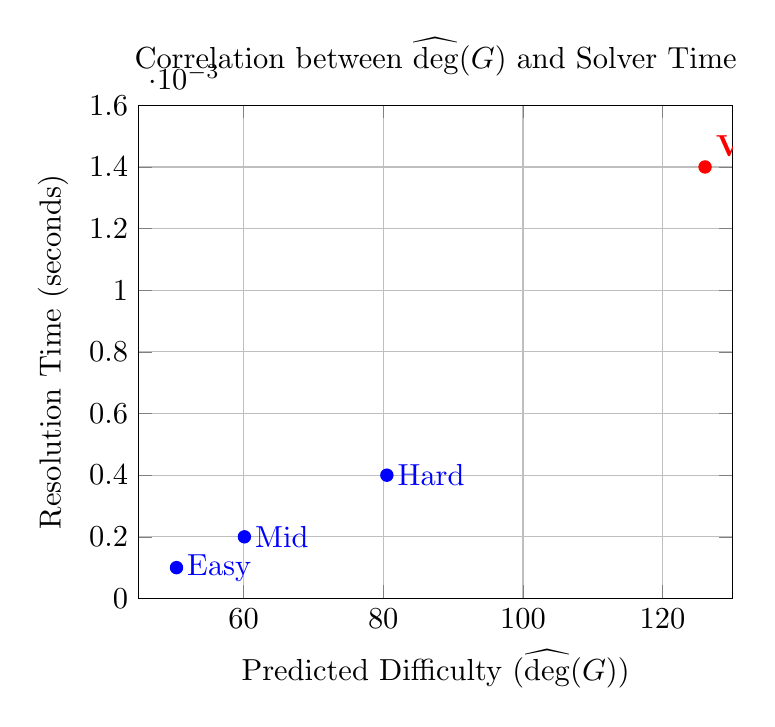
\begin{tikzpicture}[scale=1.1]
\begin{axis}[
    title={Correlation between $\hdeg(G)$ and Solver Time},
    xlabel={Predicted Difficulty ($\hdeg(G)$)},
    ylabel={Resolution Time (seconds)},
    grid=major,
    xmin=45, xmax=130,
    ymin=0, ymax=0.0016,
    ytick distance=0.0002,
    scatter/classes={
        easy={mark=*,draw=blue,fill=blue},
        mid={mark=*,draw=blue,fill=blue},
        hard={mark=*,draw=blue,fill=blue},
        vhard={mark=*,draw=red,fill=red}
    }
]
\addplot[scatter,only marks,point meta=explicit symbolic] table[meta=label] {
    x       y       label
    50.395  0.0001  easy
    60.123  0.0002  mid
    80.522  0.0004  hard
    126.084 0.0014  vhard
};

\node[anchor=west, text=blue] at (axis cs:50.395,0.0001) {Easy};
\node[anchor=west, text=blue] at (axis cs:60.123,0.0002) {Mid};
\node[anchor=west, text=blue] at (axis cs:80.522,0.0004) {Hard};
\node[anchor=south west, text=red] at (axis cs:126.084,0.0014) {\textbf{V. Hard}};

\end{axis}
\end{tikzpicture}
% ---- UPDATED (caption clarified; keeps your plot) ----
\caption{Correlation between $\hdeg(G)$ and MiniSat time (legacy illustrative data).}
\end{figure}
\FloatBarrier

% ============================
\section{Limitations and Future Directions}

\paragraph{Theoretical gaps.}
All main claims (Conjectures~\ref{conj:mpcc}--\ref{conj:pc-touch}) remain unproved.
Establishing even a partial result---for example,
$\mathrm{PC\text{-}degree}(\mathrm{Tseitin}(G)) \geq \Omega(\hdeg(G))$
for a restricted graph family---would significantly strengthen the framework.
Clarifying the relation between $\hdeg(G)$ and known measures such as Resolution
width~\cite{BenSassonWigderson2001} or treewidth is an important open direction.

\paragraph{Experimental limitations.}
The empirical validation in this preprint is limited in scope:
\begin{itemize}
  \item small instance sizes ($n \leq 80$);
  \item few data points per family (on the order of $4$--$10$ instances);
  \item no formal statistical analysis (regression, confidence intervals);
  \item no comparison with alternative predictors (e.g.\ treewidth, Resolution width,
        expansion alone, clause-learning statistics);
  \item apparent outliers (e.g.\ 6-regular $n=80$) remain unexplained;
  % ---- UPDATED (one extra safety item) ----
  \item no claim of average-case hardness or asymptotic lower bounds is made.
  \item the observed transition is reported at a single $(n,d)$ and with a fixed timeout;
      mapping its dependence on $n$, $d$, and solver settings remains future work.
\end{itemize}
A convincing validation would require: (i) at least $100$ instances per family, scaling
to $n \geq 10^3$; (ii) multiple random seeds per configuration; (iii) formal regression
analysis (e.g.\ log-time explained by $\hdeg(G)$); and (iv) head-to-head comparison with
known complexity measures.

\paragraph{Open questions.}
We highlight a few questions that we believe are both natural and approachable:
\begin{itemize}
  \item Does $\hdeg(G)$ provably lower-bound PC-degree or Resolution width for some
        nontrivial graph families?
  \item How does $\hdeg(G)$ compare empirically to treewidth or pathwidth as a hardness
        predictor across standard SAT benchmarks?
  \item Can the Kolmogorov formulation (Conjecture~\ref{conj:kmpcc}) be made rigorous
        via explicit incompressibility arguments for random or pseudorandom graph families?
\end{itemize}
We view this work as a \emph{hypothesis-generating} exercise and encourage the community
to test, extend, or refute these ideas.

% ============================
\section{Licensing}

Experimental code (Python scripts) is released under the \textbf{MIT License}.
This document and embedded figures are under the \textbf{CC BY 4.0} license.

% ============================
\begin{thebibliography}{99}

\bibitem{Landauer1961}
R.~Landauer.
\newblock Irreversibility and heat generation in the computing process.
\newblock \emph{IBM Journal of Research and Development}, 5(3):183--191, 1961.

\bibitem{Chung1997}
F.~R.~K. Chung.
\newblock \emph{Spectral Graph Theory}.
\newblock CBMS 92, American Mathematical Society, 1997.

\bibitem{Tseitin1968}
G.~Tseitin.
\newblock On the complexity of derivation in propositional calculus.
\newblock In \emph{Studies in Constructive Mathematics and Mathematical Logic},
  Part II, pages 115--125. Consultants Bureau, 1968.

\bibitem{Razborov1998}
A.~Razborov.
\newblock Lower bounds for the polynomial calculus.
\newblock \emph{Computational Complexity}, 7(4):291--324, 1998.

\bibitem{BenSassonWigderson2001}
E.~Ben-Sasson and A.~Wigderson.
\newblock Short proofs are narrow.
\newblock \emph{Journal of the ACM}, 48(2):149--169, 2001.

\bibitem{KrajicekBook}
J.~Kraj\'{\i}\v{c}ek.
\newblock \emph{Bounded Arithmetic, Propositional Logic and Complexity Theory}.
\newblock Cambridge University Press, 1995.

\bibitem{LiVitanyi}
M.~Li and P.~Vit\'{a}nyi.
\newblock \emph{An Introduction to Kolmogorov Complexity and Its Applications}.
\newblock Springer, 3rd edition, 2008.

\bibitem{HooryLinialWigderson}
S.~Hoory, N.~Linial, and A.~Wigderson.
\newblock Expander graphs and their applications.
\newblock \emph{Bulletin of the American Mathematical Society}, 43(4):439--561, 2006.

\end{thebibliography}

\end{document}
